
% !TEX program = xelatex
% 编译方式：XeLaTeX
% VSCode 推荐插件：LaTeX Workshop
% 主文件：main.tex

\documentclass[10pt,twocolumn]{ctexart}

% =========================
% 页面与版式：近似 SIGIR/ACM 双栏风格
% =========================
\usepackage[a4paper,top=1.8cm,bottom=2.0cm,left=1.55cm,right=1.55cm,columnsep=0.75cm]{geometry}
\usepackage{fontspec}
\usepackage{xeCJK}
\usepackage{amsmath,amssymb,amsfonts}
\usepackage{booktabs}
\usepackage{multirow}
\usepackage{makecell}
\usepackage{array}
\usepackage{graphicx}
\usepackage{caption}
\usepackage{subcaption}
\usepackage{float}
\usepackage{url}
\usepackage{xcolor}
\usepackage{enumitem}
\usepackage{hyperref}
\usepackage{algorithm}
\usepackage{algorithmic}
\usepackage{fancyhdr}
\usepackage{titlesec}
\usepackage{balance}
\usepackage{placeins}

\hypersetup{
  colorlinks=true,
  linkcolor=black,
  citecolor=black,
  urlcolor=blue
}

% 字体设置：Windows 下通常可用
% 如果编译报字体不存在，把 SimSun / Microsoft YaHei 改成你电脑已有字体
\setmainfont{Times New Roman}
\setsansfont{Arial}
\setmonofont{Consolas}
\setCJKmainfont{SimSun}
\setCJKsansfont{Microsoft YaHei}
\setCJKmonofont{Microsoft YaHei}

\captionsetup{font=small,labelfont=bf}

% 紧凑但稳定的双栏排版参数
\titlespacing*{\section}{0pt}{0.8em}{0.45em}
\titlespacing*{\subsection}{0pt}{0.6em}{0.25em}
\titlespacing*{\subsubsection}{0pt}{0.4em}{0.2em}
\setlength{\textfloatsep}{6pt plus 2pt minus 2pt}
\setlength{\floatsep}{6pt plus 2pt minus 2pt}
\setlength{\intextsep}{6pt plus 2pt minus 2pt}
\setlength{\abovecaptionskip}{3pt}
\setlength{\belowcaptionskip}{2pt}

\setlist[itemize]{leftmargin=1.2em,itemsep=0.2em,topsep=0.2em}
\setlist[enumerate]{leftmargin=1.2em,itemsep=0.2em,topsep=0.2em}

\titleformat{\section}{\large\bfseries}{\thesection}{0.5em}{}
\titleformat{\subsection}{\normalsize\bfseries}{\thesubsection}{0.5em}{}
\titleformat{\subsubsection}{\normalsize\itshape}{\thesubsubsection}{0.5em}{}

\raggedbottom
\pagestyle{fancy}
\fancyhf{}
\fancyhead[L]{基于可靠性感知与异构关系重排序的跨城市选址推荐}
\fancyhead[R]{深度学习课程论文}
\fancyfoot[C]{\thepage}
\renewcommand{\headrulewidth}{0.3pt}

% =========================
% 占位图宏：没有图片也能编译
% =========================
\newcommand{\figplaceholder}[2][0.95\linewidth]{
\begin{center}
\fbox{
\begin{minipage}[c][0.24\textheight][c]{#1}
\centering
\vspace{0.4em}
{\bfseries 图占位}\\[0.6em]
#2\\[0.6em]
\small 将对应 PNG/PDF 放入 figures/ 后替换为 \texttt{\textbackslash includegraphics}
\vspace{0.4em}
\end{minipage}}
\end{center}
}

\newcommand{\tabplaceholder}[1]{
\begin{center}
\fbox{
\begin{minipage}{0.95\linewidth}
\centering
{\bfseries 表格占位}\\[0.5em]
#1\\[0.5em]
\small 后续可由 CSV 转 LaTeX 表格替换。
\end{minipage}}
\end{center}
}

\title{\bfseries 基于可靠性感知安全迁移与异构关系重排序的跨城市选址推荐研究}

\author{
郭丞浩\\
山东大学软件学院\\
学号：\texttt{202400300319}\\
邮箱：\texttt{2139865291@qq.com}
}

\date{}

\begin{document}
\maketitle

\begin{abstract}
商业选址推荐旨在为品牌预测适合开设新门店的城市区域，是现代商业决策中的重要任务。与传统推荐系统相比，选址推荐面临更严重的数据稀疏问题：单个品牌在一个城市中的门店数量通常较少，不同城市之间又存在商业结构、消费习惯和区域功能的显著差异。已有 Optimal Transport enhanced Cross-city（OTC）方法通过 Gromov-Wasserstein 最优传输将源城市的品牌与区域表示投影到目标城市，从而利用跨城市信息缓解目标城市数据不足问题。然而，原始 OTC 框架隐含假设来自其他城市的迁移信号总体有益，缺少对源城市可靠性和负迁移风险的显式控制。本文首先在 OpenSiteRec 数据集上复现 OTC-GW 框架，并观察到无回退跨城市融合在多个设置下会低于目标城市本地模型。基于该现象，本文提出 RD-Safe+HR-OTC 框架：其中，RD-Safe 模块通过源城市可靠性估计与安全门控抑制负迁移；HR-Rerank 模块进一步利用类别--区域亲和力、区域共现扩散和区域热度先验等异构商业结构信号对候选区域进行重排序。实验结果表明，在 MF backbone 上，所提方法显著优于 Target-only 和 Original OTC-GW；在 LightGCN backbone 上，所提方法主要表现为修复无回退 OTC-GW 的负迁移，并接近强本地图模型的性能。此外，本文进一步进行了完整消融实验和 strict unseen-pair 鲁棒性分析，以验证各模块的作用和更严格评价场景下的泛化能力。
\end{abstract}

\noindent\textbf{关键词：}选址推荐；跨城市推荐；最优传输；负迁移；异构图重排序；可靠性感知迁移

\section{引言}

商业选址推荐（site recommendation）旨在预测品牌适合开设新门店的城市区域。对于真实商业决策而言，合适的选址可能带来显著收益，而错误的选址则可能导致经营失败。因此，如何利用数据驱动方法辅助品牌进行选址决策，是推荐系统、城市计算和商业智能交叉领域中的重要问题。

与传统推荐任务相比，选址推荐具有明显不同的特点。传统推荐系统通常拥有大规模用户行为，而选址推荐面对的是品牌与城市区域之间的交互关系。一个品牌在单个城市中往往只有少量门店，导致品牌--区域交互矩阵极度稀疏。原始 OTC 论文指出，OpenSiteRec 数据集中每个品牌平均仅有约 5 个站点，不同城市在类别分布、品牌分布和区域分布上也存在显著差异。这种稀疏性和跨城市差异使得仅依赖目标城市本地数据的模型容易学习不充分。

为缓解这一问题，原始 OTC 方法提出利用其他城市的数据增强目标城市选址推荐。其核心思想是：先在每个城市中训练单城市推荐 backbone，得到品牌与区域 embedding；再利用 Gromov-Wasserstein 最优传输分别对齐源城市与目标城市的品牌空间和区域空间，将源城市推荐信号投影到目标城市；最后将目标城市本地推荐分数与多个源城市的迁移分数进行加权融合。该框架为选址推荐提供了一种轻量级跨城市迁移方案。

然而，跨城市迁移并不天然可靠。不同城市之间可能存在商业结构、城市规划、消费习惯和品牌布局差异。若某个源城市与目标城市不匹配，直接融合其迁移分数可能破坏本地模型已经学到的排序结果，即产生负迁移。本文在复现无回退 OTC-GW 时也观察到这一现象：当融合权重不允许退回到本地模型时，Original OTC-GW 在 MF 和 LightGCN 两类 backbone 上均可能低于 Target-only。

基于上述发现，本文提出 RD-Safe+HR-OTC 框架。RD-Safe 模块从“迁移是否可靠”的角度出发，根据内部验证集估计源城市贡献，并通过安全门控决定是否采用迁移结果；HR-Rerank 模块从“商业结构是否充分利用”的角度出发，在基础推荐分数之上加入类别--区域亲和力、区域共现扩散和区域热度先验三类异构关系信号，对最终候选区域进行重排序。

本文主要贡献如下：
\begin{itemize}
  \item 对 OTC-GW 跨城市选址推荐框架进行复现，并在无回退设置下观察到跨城市迁移可能导致明显负迁移。
  \item 提出 RD-Safe 可靠性感知安全迁移策略，通过源城市可靠性筛选和安全门控缓解不可靠源城市带来的负迁移。
  \item 提出 HR-Rerank 异构关系重排序策略，将类别--区域亲和力、区域共现扩散和区域热度先验引入最终排序，使推荐结果更符合商业选址中的结构规律。
  \item 在 OpenSiteRec 四城市数据集上进行三 seed 实验、完整消融实验和 strict unseen-pair 鲁棒性分析，验证所提方法的有效性与局限。
\end{itemize}

\section{预备知识与问题定义}

\subsection{OpenSiteRec 数据集}

本文使用 OpenSiteRec 数据集进行实验。该数据集包含 Chicago、New York City、Singapore 和 Tokyo 四个国际城市的真实商业实体。根据原始论文，OpenSiteRec 中包括五类实体：Brand、Category、POI、Business Area 和 Region。其中，Brand 表示商业品牌或机构，Category 表示门店类别，POI 表示具体站点，Region 表示城市行政或地理区域，Business Area 表示商业区域。

在 vanilla setting 下，原始 OTC 主要使用 Brand、POI 和 Region 三部分信息，将选址推荐建模为品牌到区域的 Top-$N$ 推荐任务。本文延续该基本任务设定，并在 HR-Rerank 中额外使用训练集中可获得的类别和区域关系构造轻量级异构结构信号。

\begin{table}[H]
\centering
\caption{OpenSiteRec 数据集统计。}
\label{tab:dataset_stats}
\begin{tabular}{lrrr}
\toprule
City & Brand & Region & Site \\
\midrule
Chicago & 969 & 801 & 8,044 \\
New York City & 2,702 & 2,325 & 14,189 \\
Singapore & 1,922 & 2,043 & 9,912 \\
Tokyo & 4,861 & 3,036 & 26,765 \\
\bottomrule
\end{tabular}
\end{table}

\subsection{选址推荐任务定义}

给定城市中的品牌集合 $\mathcal{U}=\{u_1,u_2,\ldots,u_M\}$ 和区域集合 $\mathcal{V}=\{v_1,v_2,\ldots,v_N\}$，可以构造品牌--区域交互矩阵 $P\in \{0,1\}^{M\times N}$。若品牌 $u_i$ 在区域 $v_j$ 中存在至少一个 POI，则 $P_{ij}=1$，否则 $P_{ij}=0$。选址推荐的目标是对每个品牌预测其可能适合开店的区域列表，即学习预测矩阵 $\hat{P}$ 并进行 Top-$N$ 排序。

在跨城市场景下，给定目标城市 $t$ 以及若干源城市集合 $\mathcal{S}=\{s_1,s_2,\ldots,s_K\}$，目标是利用源城市中的品牌--区域分布信息，提升目标城市的选址推荐效果。

\subsection{Gromov-Wasserstein 最优传输}

最优传输（Optimal Transport, OT）用于学习两个分布之间的最优对齐关系。在跨城市选址推荐中，由于不同城市的品牌集合和区域集合并不完全一致，且区域空间完全不同，普通 Wasserstein 距离难以直接应用。Gromov-Wasserstein（GW）距离通过对齐域内结构关系而非直接对齐实例特征，更适合这种跨域场景。

设源城市与目标城市中品牌或区域的嵌入表示分别为 $\hat{X}^{s}$ 与 $\hat{X}^{t}$，GW 通过最小化两域内部距离结构差异学习传输计划 $T^{st}$。该传输计划可用于将源城市 embedding 投影到目标城市，从而得到跨城市迁移推荐分数。

\section{原始 OTC 方法复现与问题分析}

\subsection{单城市推荐 Backbone}

OTC 框架首先在每个城市中训练单城市推荐 backbone。给定品牌 $u$ 和区域 $v$，模型将二者映射为 $d$ 维 embedding：
\begin{equation}
    \mathbf{u}, \mathbf{v} = \mathrm{Embed}(u,v).
\end{equation}
不同 backbone 可以采用不同交互层。对于 MF，交互层可以视为恒等映射；对于 LightGCN，则通过品牌--区域二部图上的邻居聚合学习高阶协同信号。最终预测分数通常由内积得到：
\begin{equation}
    \hat{P}_{uv} = \hat{\mathbf{u}}^\top \hat{\mathbf{v}}.
\end{equation}

训练目标采用 BPR 损失：
\begin{equation}
    \mathcal{L} =
    -\sum_{u\in \mathcal{U}}\sum_{v\in \mathcal{N}_u}\sum_{v'\notin \mathcal{N}_u}
    \ln \sigma(\hat{P}_{uv}-\hat{P}_{uv'})
    + \lambda \|\Theta\|_2^2.
\end{equation}

\subsection{OTC-GW 跨城市迁移}

原始 OTC 对每个源城市 $s$ 和目标城市 $t$ 分别计算品牌传输计划 $T_u^{st}$ 和区域传输计划 $T_v^{st}$，然后将源城市的品牌和区域表示投影到目标城市：
\begin{equation}
    \hat{\mathbf{u}}_{j}^{st} = \sum_{i=1}^{M_s} T^{st}_{u,ij}\hat{\mathbf{u}}_{i}^{s},
\end{equation}
\begin{equation}
    \hat{\mathbf{v}}_{j}^{st} = \sum_{i=1}^{N_s} T^{st}_{v,ij}\hat{\mathbf{v}}_{i}^{s}.
\end{equation}

由投影后的品牌和区域 embedding 可得到源城市到目标城市的迁移推荐分数：
\begin{equation}
    \hat{P}^{st}_{ij} = (\hat{\mathbf{u}}^{st}_{i})^\top \hat{\mathbf{v}}^{st}_{j}.
\end{equation}

多源城市融合时，目标城市最终预测为：
\begin{equation}
    \bar{P}^{t}_{ij}
    =
    \hat{P}^{t}_{ij}
    +
    \sum_{k=1}^{K}\gamma_{s_k t}\hat{P}^{s_k t}_{ij}.
\end{equation}

\subsection{复现中发现的负迁移问题}

原始 OTC 的核心假设是源城市可以向目标城市提供有益知识。然而在实际复现中，本文发现该假设并不总是成立。若不允许 $\gamma=0$ 回退到本地模型，则 Original OTC-GW 在多个设置下会低于 Target-only。该现象说明，跨城市迁移信号可能包含噪声，尤其当源城市与目标城市商业结构差异较大时，不可靠迁移会破坏本地模型已经学习到的排序结果。


\begin{table}[H]
\centering
\caption{Target-only 与无回退 OTC-GW 的四城市平均结果。}
\label{tab:negative_transfer}
\small
\setlength{\tabcolsep}{3pt}
\resizebox{\linewidth}{!}{%
\begin{tabular}{llcc}
\toprule
Backbone & Setting & Recall@20 & nDCG@20 \\
\midrule
MF & Target & 0.2233$\pm$0.0008 & 0.1251$\pm$0.0012 \\
MF & OTC-GW & 0.2040$\pm$0.0054 & 0.1170$\pm$0.0026 \\
LightGCN & Target & 0.2809$\pm$0.0057 & 0.1741$\pm$0.0026 \\
LightGCN & OTC-GW & 0.2286$\pm$0.0037 & 0.1291$\pm$0.0029 \\
\bottomrule
\end{tabular}%
}
\vspace{0.2em}

\begin{minipage}{0.96\linewidth}
\scriptsize 注：Target 表示仅使用目标城市训练的本地模型；OTC-GW 表示无回退 Original-OTC-GW-NoFallback。结果为四城市平均 mean$\pm$std。
\end{minipage}
\end{table}



\begin{figure}[H]
\centering
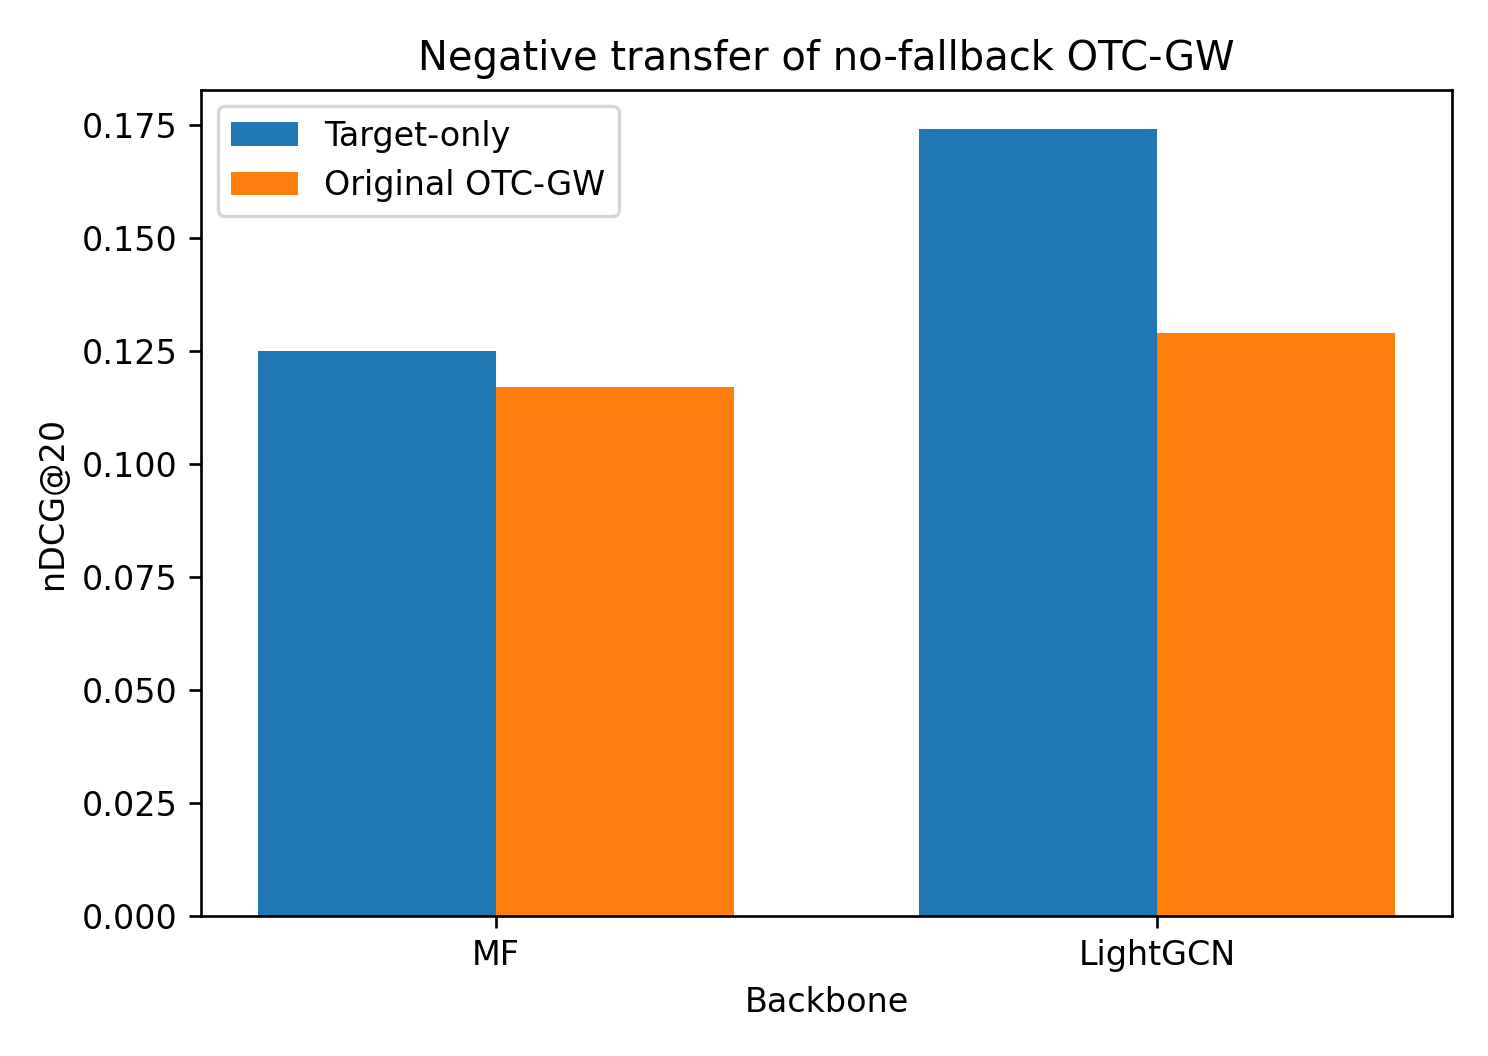
\includegraphics[width=\linewidth]{figures/fig_negative_transfer_ndcg.png}
\caption{无回退 Original OTC-GW 相比 Target-only 的负迁移现象。}
\label{fig:negative_transfer}
\end{figure}


\section{方法}

\subsection{总体框架}

本文提出 RD-Safe+HR-OTC 框架。整体流程如图~\ref{fig:framework} 所示。首先，在目标城市和源城市上分别训练单城市 backbone，并使用 OTC-GW 得到跨城市迁移分数。其次，RD-Safe 根据内部验证集估计源城市可靠性，并通过安全门控决定是否采用迁移分数。最后，HR-Rerank 利用目标城市训练集中的异构商业关系构造三类结构信号，对基础推荐分数进行重排序。



\begin{figure*}[t]
\centering
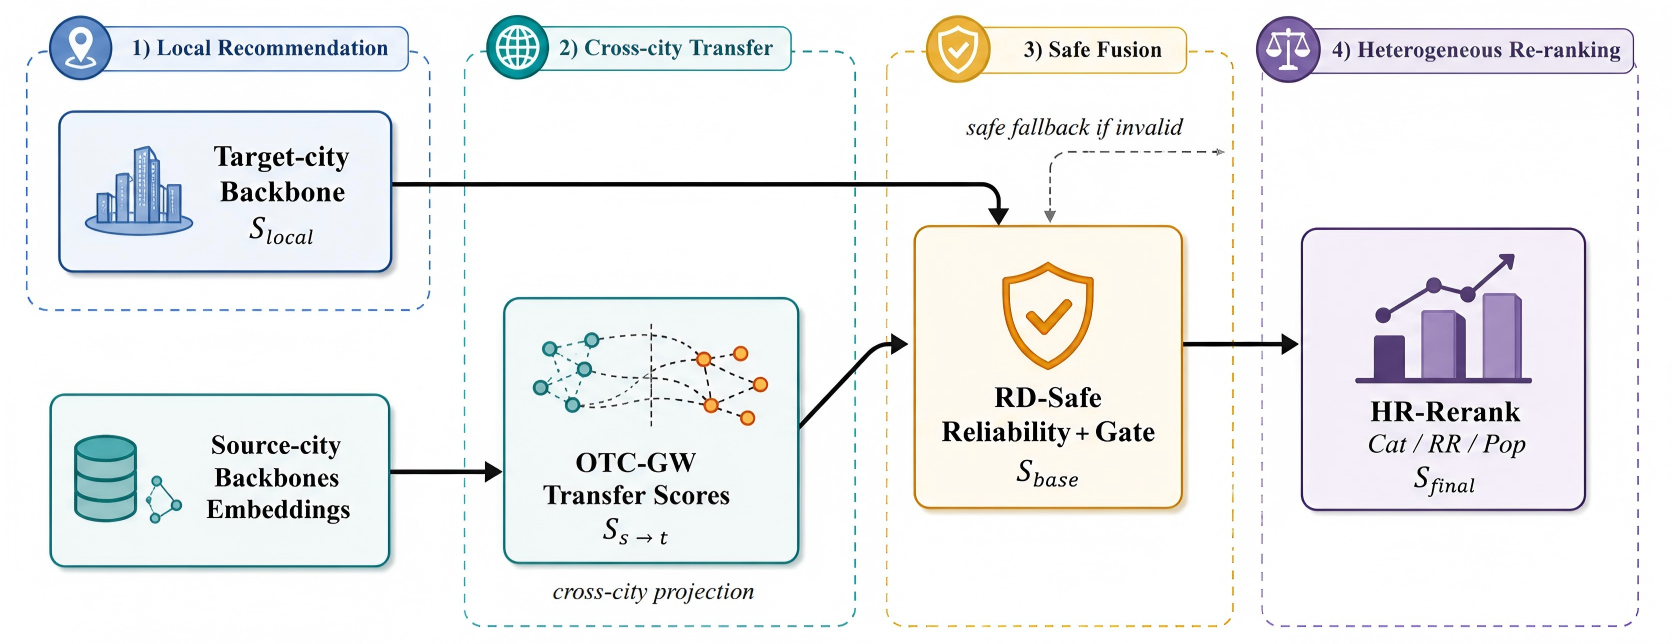
\includegraphics[width=0.82\textwidth]{figures/fig_framework.png}
\caption{RD-Safe+HR-OTC 总体框架。}
\label{fig:framework}
\end{figure*}



\subsection{RD-Safe：可靠性感知安全迁移}

RD-Safe 的目标是缓解 Original OTC-GW 中不可靠源城市带来的负迁移。与直接融合所有源城市迁移分数不同，RD-Safe 首先在内部验证集上评估每个源城市的单源迁移效果，只有当迁移在 nDCG@20 上带来足够提升且不明显损害 Recall@20 时，才将该源城市视为可靠源城市。

设目标城市本地分数为 $S_{\mathrm{local}}$，源城市 $s$ 到目标城市的迁移分数为 $S_{s\rightarrow t}$。对于每个源城市，RD-Safe 在候选权重集合 $\mathcal{B}$ 中搜索：
\begin{equation}
    S_{s}^{\mathrm{single}} = S_{\mathrm{local}} + \beta S_{s\rightarrow t},\quad \beta\in \mathcal{B}.
\end{equation}
若该源城市在验证集上的最优结果满足：
\begin{equation}
    \Delta \mathrm{nDCG}@20 \geq \epsilon_{\mathrm{src}},
    \quad
    \Delta \mathrm{Recall}@20 \geq -\epsilon_{\mathrm{rec}},
\end{equation}
则将其加入可靠源城市集合。

对于多个可靠源城市，本文根据其验证集 nDCG 增益构造归一化源城市权重：
\begin{equation}
    w_s = \frac{\max(\Delta_s,0)}{\sum_{s'\in \mathcal{R}}\max(\Delta_{s'},0)}.
\end{equation}
由此得到可靠源城市加权迁移分数：
\begin{equation}
    S_{\mathrm{RD}} = \sum_{s\in \mathcal{R}}w_s S_{s\rightarrow t}.
\end{equation}

最终，RD-Safe 在 Local、Original OTC 和 RD 迁移候选之间进行安全选择。若 RD 候选没有在验证集上超过安全基线，或导致 Recall 下降，则回退到更安全的候选分数。该策略使模型不会强制采用不可靠迁移，从而降低负迁移风险。

\begin{algorithm}[H]
\caption{RD-Safe 可靠性感知安全迁移}
\label{alg:rdsafe}
\begin{algorithmic}[1]
\REQUIRE Local score $S_{\mathrm{local}}$, transfer scores $\{S_{s\rightarrow t}\}$, validation set $\mathcal{D}_{val}$
\STATE Evaluate $S_{\mathrm{local}}$ on $\mathcal{D}_{val}$
\FOR{each source city $s$}
    \STATE Tune $\beta$ for $S_{\mathrm{local}}+\beta S_{s\rightarrow t}$ on $\mathcal{D}_{val}$
    \STATE Add $s$ into reliable set $\mathcal{R}$ if validation gain is reliable
\ENDFOR
\STATE Construct weighted reliable transfer $S_{\mathrm{RD}}=\sum_{s\in\mathcal{R}}w_sS_{s\rightarrow t}$
\STATE Tune final fusion candidates on $\mathcal{D}_{val}$
\STATE Return the candidate only if it passes the safety gate; otherwise fallback
\end{algorithmic}
\end{algorithm}

\subsection{HR-Rerank：异构关系重排序}

RD-Safe 主要解决迁移是否可靠的问题，但它仍然基于已有推荐分数进行选择。为了进一步利用商业选址中的结构规律，本文提出 HR-Rerank，在基础推荐分数上加入三类异构关系信号。

给定基础分数 $S_{\mathrm{base}}$，HR-Rerank 的最终分数为：
\begin{equation}
\begin{split}
S_{\mathrm{final}}(b,r)
=
&~\mathrm{Norm}(S_{\mathrm{base}}(b,r)) \\
&+ \lambda_c S_{\mathrm{cat}}(b,r)
+ \lambda_{rr}S_{\mathrm{rr}}(b,r)
+ \lambda_p S_{\mathrm{pop}}(r),
\end{split}
\end{equation}
其中，$b$ 表示品牌，$r$ 表示候选区域，$S_{\mathrm{cat}}$ 为类别--区域亲和力，$S_{\mathrm{rr}}$ 为区域共现扩散，$S_{\mathrm{pop}}$ 为区域热度先验。

\subsubsection{类别--区域亲和力}

类别--区域亲和力刻画某一类品牌与某一区域之间的适配程度。其商业直觉是，不同业态适合的区域不同。例如，咖啡店可能更适合办公区和商业区，酒店可能更适合交通枢纽或旅游区域。本文根据训练集中各类别品牌在不同区域的出现频率构造该信号。若目标品牌所属类别在某个区域中频繁出现，则该区域对该类别品牌具有更高亲和力。

\subsubsection{区域共现扩散}

区域共现扩散刻画候选区域与品牌已有区域之间的关系。若两个区域经常被相同品牌共同选择，则说明它们在商业选址上可能具有相似性。本文根据训练集中的品牌--区域交互构建区域--区域共现矩阵，并将品牌已知区域的偏好沿区域关系扩散到候选区域。该信号尤其有助于低支持品牌，因为品牌自身历史样本较少，但区域共现图能够提供额外结构信息。

\subsubsection{区域热度先验}

区域热度先验刻画某个区域整体商业活跃程度。本文使用训练集中区域承载的 POI 或品牌数量近似区域热度，并对其进行归一化后加入最终重排序。需要注意的是，区域热度只作为弱先验，并不替代个性化推荐。若验证集显示该信号无益，其权重会被调低或被安全门控回退。

\subsection{验证集选择与安全门控}

HR-Rerank 的参数 $\lambda_c,\lambda_{rr},\lambda_p$ 在内部验证集上进行搜索。若图重排序未能带来足够 nDCG@20 提升，或导致 Recall@20 下降，则回退到对应的基础分数。该门控机制与 RD-Safe 的思想一致，即宁可保持安全基线，也不强行引入不稳定增强。

\section{实验}

\subsection{实验设置}

\subsubsection{数据集与划分}

本文在 OpenSiteRec 四城市数据集上进行实验，包括 Chicago、New York City、Singapore 和 Tokyo。实验采用官方训练/测试划分，并进一步从训练集中划分内部验证集用于参数选择。所有最终结果在测试集上报告。

\subsubsection{评价指标}

本文采用 Top-$N$ 推荐中常用的 Recall@20 和 nDCG@20 作为评价指标。Recall@20 衡量测试集中正样本被 Top-20 推荐列表命中的比例，nDCG@20 进一步考虑命中位置，能够衡量推荐列表整体排序质量。

\subsubsection{比较方法}

本文比较以下方法：
\begin{itemize}
    \item \textbf{Target-only}：仅使用目标城市训练数据训练单城市推荐模型。
    \item \textbf{Original-OTC-GW-NoFallback}：无回退 OTC-GW，融合权重 $\gamma$ 不包含 0。
    \item \textbf{RD-Safe-OTC-GW}：在 OTC-GW 基础上加入可靠源城市筛选与安全门控。
    \item \textbf{HR-Rerank-OTC-GW}：在 Original OTC-GW 基础上加入异构关系重排序。
    \item \textbf{RD-Safe+HR-Rerank-OTC-GW}：本文完整方法。
\end{itemize}

本文选择 VanillaMF 和 LightGCN 作为 backbone。所有主要实验均使用 2024、2025 和 2026 三个随机种子，并报告 mean$\pm$std。

\subsection{主实验结果}


从表~\ref{tab:main_results} 可以看出，在 MF backbone 上，RD-Safe+HR-OTC 在四个城市上均取得最优或接近最优结果，四城市平均 Recall@20 和 nDCG@20 分别达到 0.2666 和 0.1598，明显高于 Target-only 的 0.2233 和 0.1251。这说明当本地模型表达能力有限时，可靠迁移和异构关系重排序能够提供有效补充。相比之下，在 LightGCN backbone 上，Target-only 已经达到 0.2809/0.1741 的四城市平均性能，RD-Safe+HR-OTC 为 0.2808/0.1738，基本与本地 LightGCN 持平。该现象表明，LightGCN 已通过图传播捕获较强高阶结构，HR-Rerank 中的部分图结构信号与其存在重叠。

\begin{table*}[!t]
\centering
\caption{OpenSiteRec 官方测试集上的主实验结果，报告三次随机种子 mean$\pm$std。每个 backbone 下最优结果加粗。}
\label{tab:main_results}
\resizebox{\textwidth}{!}{%
\begin{tabular}{llcccccccc}
\toprule
\multirow{2}{*}{Backbone} & \multirow{2}{*}{Method} & \multicolumn{2}{c}{Chicago} & \multicolumn{2}{c}{New York City} & \multicolumn{2}{c}{Singapore} & \multicolumn{2}{c}{Tokyo} \\
\cmidrule(lr){3-4}\cmidrule(lr){5-6}\cmidrule(lr){7-8}\cmidrule(lr){9-10}
& & Rec@20 & nDCG@20 & Rec@20 & nDCG@20 & Rec@20 & nDCG@20 & Rec@20 & nDCG@20 \\
\midrule
MF & Target-only & 0.1950$\pm$0.0061 & 0.1327$\pm$0.0037 & 0.1253$\pm$0.0033 & 0.0619$\pm$0.0008 & 0.4478$\pm$0.0003 & 0.2391$\pm$0.0020 & 0.1253$\pm$0.0007 & 0.0667$\pm$0.0005\\
 & Original OTC-GW & 0.1366$\pm$0.0292 & 0.1090$\pm$0.0120 & 0.1192$\pm$0.0137 & 0.0600$\pm$0.0047 & 0.4355$\pm$0.0155 & 0.2322$\pm$0.0050 & 0.1247$\pm$0.0019 & 0.0668$\pm$0.0005\\
 & RD-Safe-OTC & 0.1932$\pm$0.0091 & 0.1323$\pm$0.0041 & 0.1263$\pm$0.0049 & 0.0624$\pm$0.0016 & 0.4478$\pm$0.0003 & 0.2391$\pm$0.0020 & 0.1253$\pm$0.0007 & 0.0667$\pm$0.0005\\
 & HR-OTC & 0.2270$\pm$0.0068 & 0.1602$\pm$0.0046 & 0.1683$\pm$0.0021 & 0.0965$\pm$0.0009 & 0.4831$\pm$0.0063 & 0.2757$\pm$0.0052 & 0.1657$\pm$0.0012 & 0.0914$\pm$0.0007\\
 & RD-Safe+HR-OTC & \textbf{0.2330$\pm$0.0014} & \textbf{0.1640$\pm$0.0017} & \textbf{0.1744$\pm$0.0029} & \textbf{0.0992$\pm$0.0026} & \textbf{0.4929$\pm$0.0064} & \textbf{0.2839$\pm$0.0050} & \textbf{0.1659$\pm$0.0009} & \textbf{0.0922$\pm$0.0007}\\
 & \%Improv. to MF & +19.51\% & +23.60\% & +39.24\% & +60.33\% & +10.08\% & +18.75\% & +32.37\% & +38.21\%\\
 & \%Improv. to Original OTC & +70.60\% & +50.42\% & +46.39\% & +65.48\% & +13.18\% & +22.26\% & +33.07\% & +37.99\%\\
\midrule
LightGCN & Target-only & \textbf{0.2762$\pm$0.0092} & \textbf{0.2044$\pm$0.0041} & \textbf{0.2020$\pm$0.0094} & \textbf{0.1151$\pm$0.0020} & 0.4694$\pm$0.0101 & 0.2640$\pm$0.0055 & \textbf{0.1759$\pm$0.0054} & \textbf{0.1131$\pm$0.0012}\\
 & Original OTC-GW & 0.2454$\pm$0.0069 & 0.1581$\pm$0.0080 & 0.1222$\pm$0.0087 & 0.0650$\pm$0.0078 & 0.4111$\pm$0.0169 & 0.2183$\pm$0.0076 & 0.1359$\pm$0.0069 & 0.0749$\pm$0.0043\\
 & RD-Safe-OTC & \textbf{0.2762$\pm$0.0092} & \textbf{0.2044$\pm$0.0041} & \textbf{0.2020$\pm$0.0094} & \textbf{0.1151$\pm$0.0020} & 0.4632$\pm$0.0058 & 0.2552$\pm$0.0124 & \textbf{0.1759$\pm$0.0054} & \textbf{0.1131$\pm$0.0012}\\
 & HR-OTC & 0.2533$\pm$0.0023 & 0.1775$\pm$0.0006 & 0.1826$\pm$0.0056 & 0.1018$\pm$0.0009 & \textbf{0.4860$\pm$0.0076} & \textbf{0.2898$\pm$0.0044} & 0.1668$\pm$0.0033 & 0.1005$\pm$0.0016\\
 & RD-Safe+HR-OTC & \textbf{0.2762$\pm$0.0092} & \textbf{0.2044$\pm$0.0041} & \textbf{0.2020$\pm$0.0094} & \textbf{0.1151$\pm$0.0020} & 0.4690$\pm$0.0157 & 0.2627$\pm$0.0238 & \textbf{0.1759$\pm$0.0054} & \textbf{0.1131$\pm$0.0012}\\
 & \%Improv. to LightGCN & +0.00\% & +0.00\% & +0.00\% & +0.00\% & -0.09\% & -0.51\% & +0.00\% & +0.00\%\\
 & \%Improv. to Original OTC & +12.58\% & +29.28\% & +65.32\% & +77.11\% & +14.09\% & +20.32\% & +29.44\% & +51.02\%\\
\bottomrule
\end{tabular}%
}
\end{table*}

\begin{figure}[H]
\centering
\begin{subfigure}{0.48\linewidth}
\centering
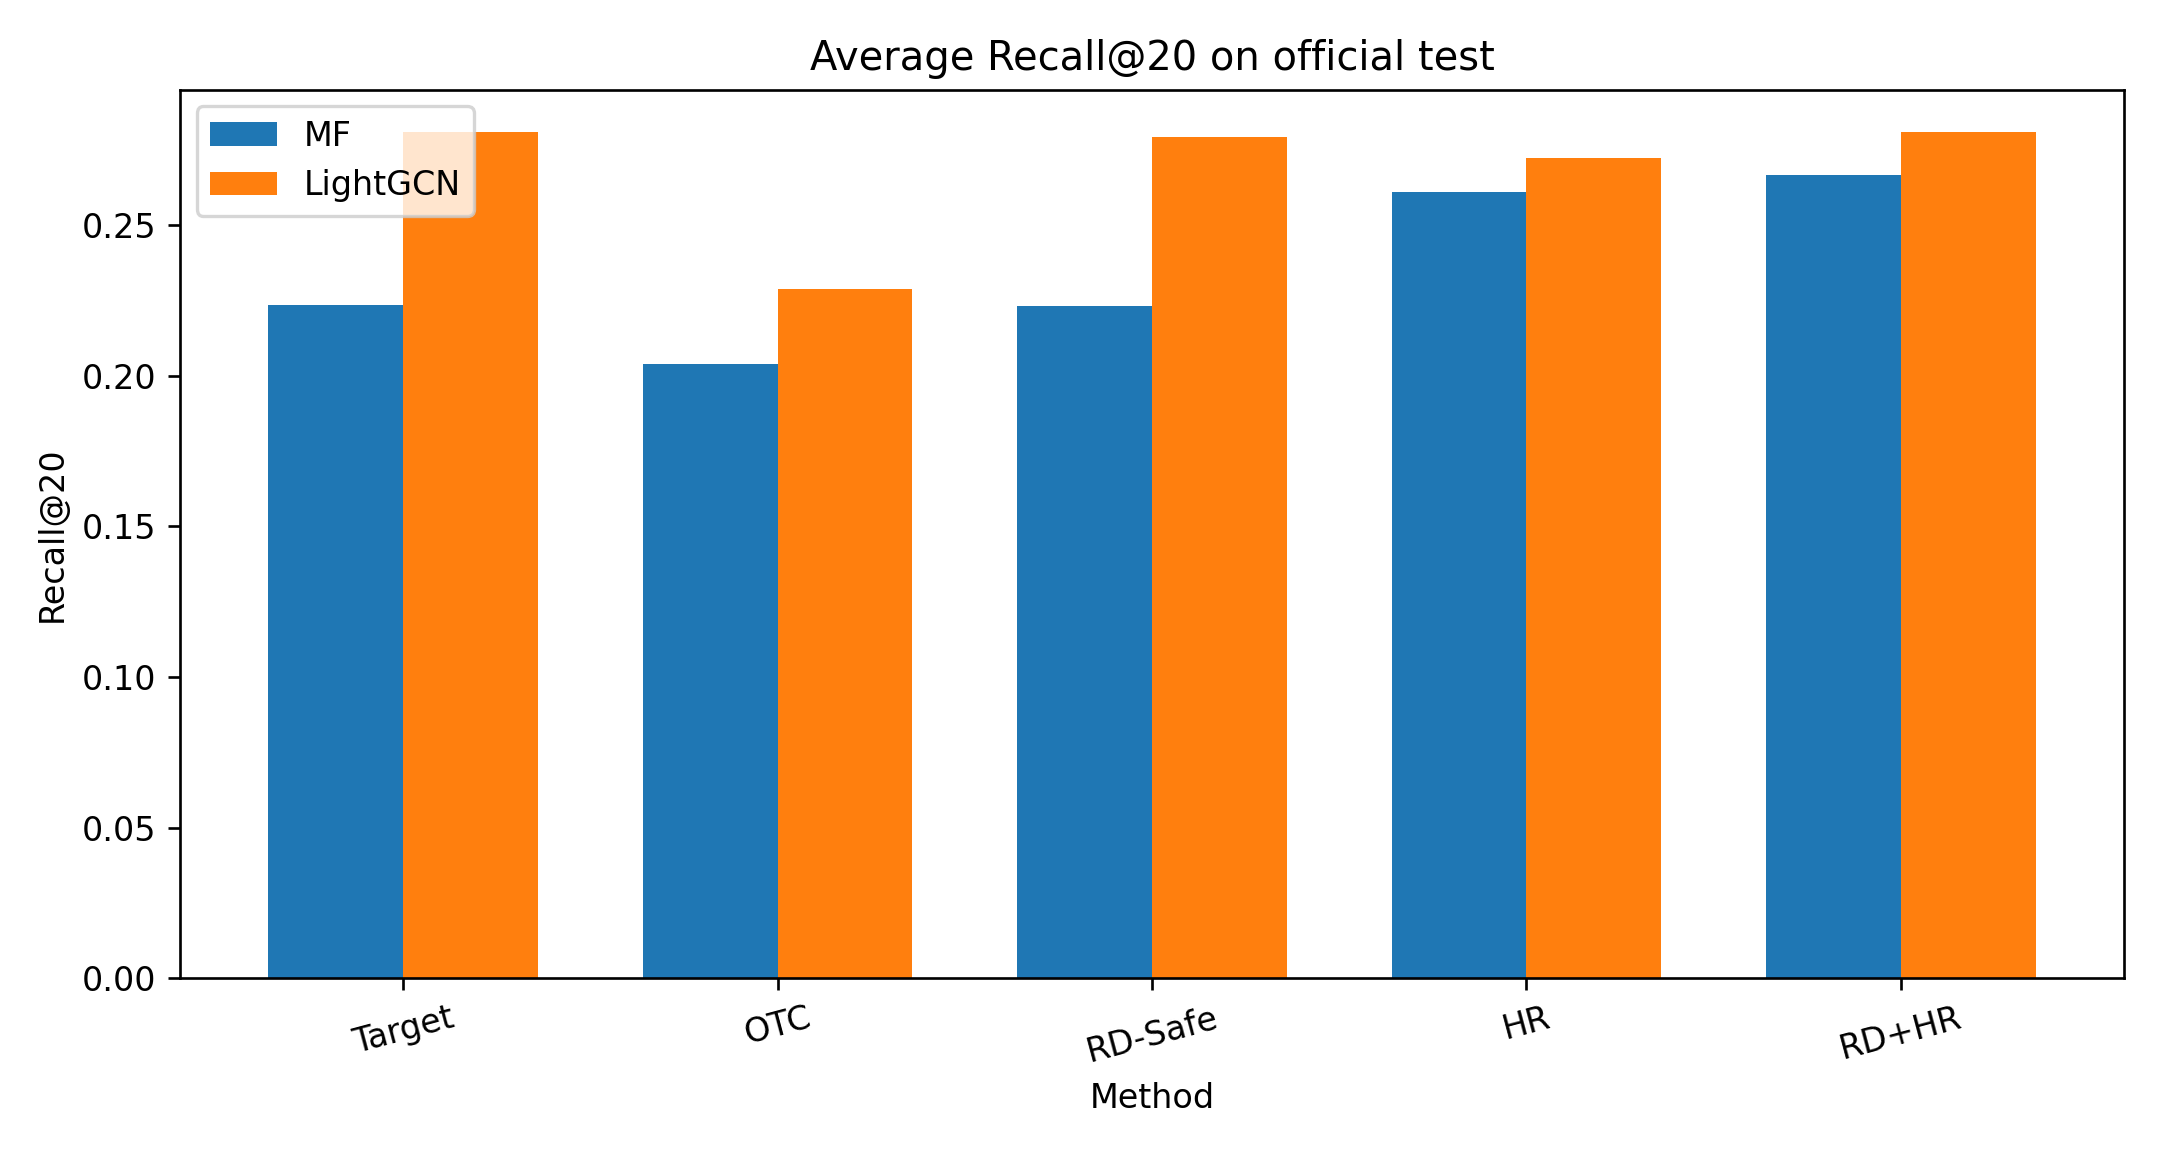
\includegraphics[width=\linewidth]{figures/fig_main_avg_recall.png}
\caption{Average Recall@20}
\end{subfigure}
\hfill
\begin{subfigure}{0.48\linewidth}
\centering
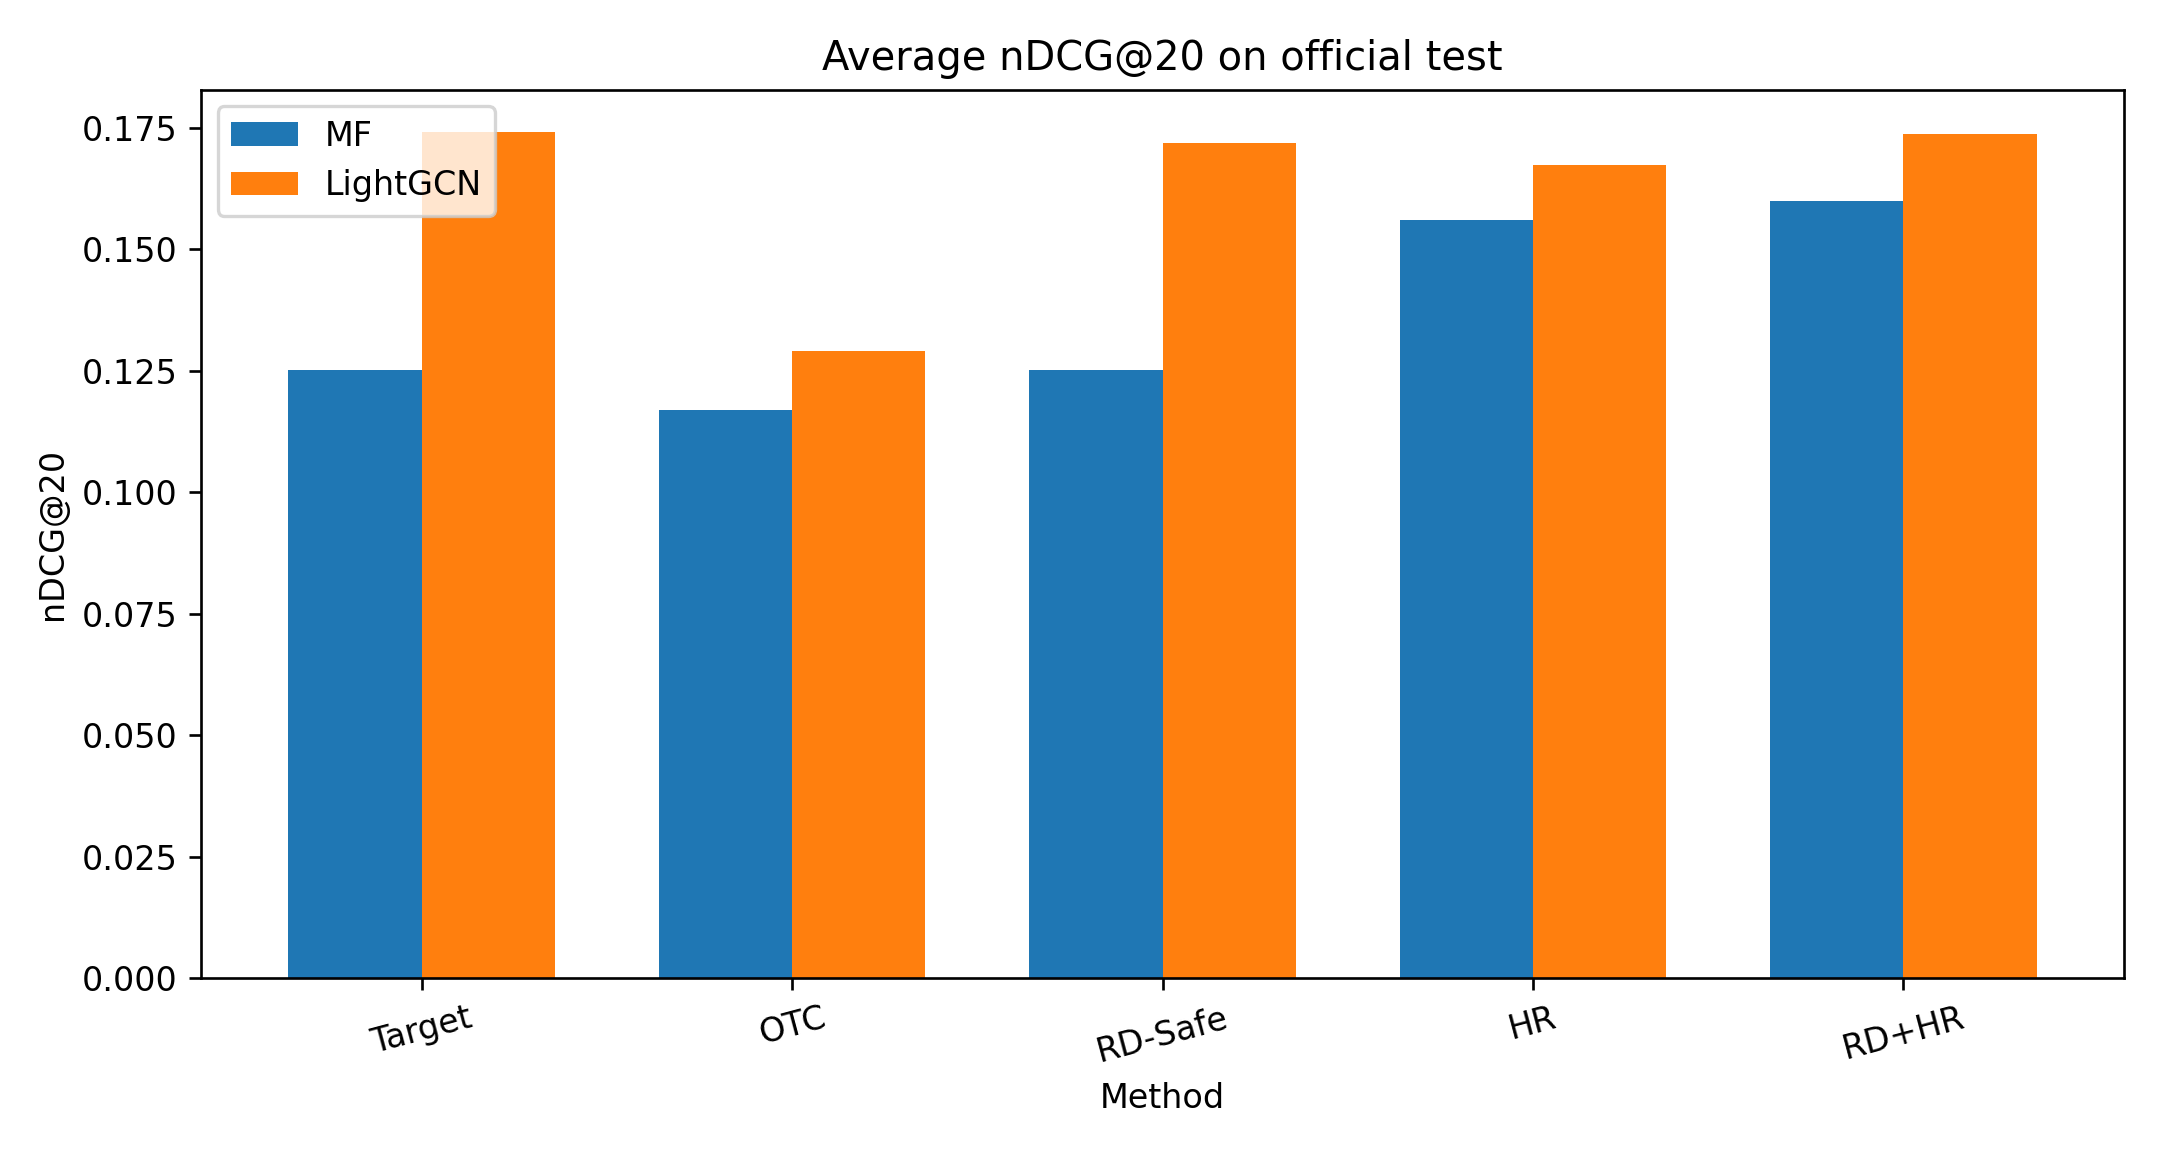
\includegraphics[width=\linewidth]{figures/fig_main_avg_ndcg.png}
\caption{Average nDCG@20}
\end{subfigure}
\caption{OpenSiteRec official test 上不同方法的四城市平均性能。柱状图展示三次随机种子的均值。}
\label{fig:main_bar}
\end{figure}

\FloatBarrier

\subsection{消融实验}

为了进一步分析各模块贡献，本文进行两组消融实验。第一组为主模块消融，用于比较 Target-only、Original OTC-GW、RD-Safe-OTC、HR-Rerank-OTC 和完整 RD-Safe+HR-OTC。第二组为 HR 内部信号消融，用于分析类别--区域亲和力、区域共现扩散和区域热度先验三类信号的贡献。

\begin{table}[H]
\centering
\caption{主模块消融实验：四城市 official test 平均结果。}
\label{tab:component_ablation}
\resizebox{\linewidth}{!}{%
\begin{tabular}{lcccc}
\toprule
\multirow{2}{*}{Method} & \multicolumn{2}{c}{MF} & \multicolumn{2}{c}{LightGCN}\\
\cmidrule(lr){2-3}\cmidrule(lr){4-5}
& Rec@20 & nDCG@20 & Rec@20 & nDCG@20\\
\midrule
Target-only & 0.2233$\pm$0.0008 & 0.1251$\pm$0.0012 & 0.2809$\pm$0.0057 & 0.1741$\pm$0.0026\\
Original OTC-GW & 0.2040$\pm$0.0054 & 0.1170$\pm$0.0026 & 0.2286$\pm$0.0037 & 0.1291$\pm$0.0029\\
RD-Safe-OTC & 0.2232$\pm$0.0010 & 0.1251$\pm$0.0012 & 0.2794$\pm$0.0034 & 0.1719$\pm$0.0016\\
HR-OTC & 0.2610$\pm$0.0013 & 0.1560$\pm$0.0019 & 0.2721$\pm$0.0028 & 0.1674$\pm$0.0010\\
RD-Safe+HR-OTC & 0.2666$\pm$0.0019 & 0.1598$\pm$0.0010 & 0.2808$\pm$0.0044 & 0.1738$\pm$0.0047\\
\bottomrule
\end{tabular}%
}
\end{table}

\begin{table}[H]
\centering
\caption{HR-Rerank 内部信号消融：四城市 official test 平均结果。}
\label{tab:hr_ablation}
\resizebox{\linewidth}{!}{%
\begin{tabular}{lcccc}
\toprule
\multirow{2}{*}{Variant} & \multicolumn{2}{c}{MF} & \multicolumn{2}{c}{LightGCN}\\
\cmidrule(lr){2-3}\cmidrule(lr){4-5}
& Rec@20 & nDCG@20 & Rec@20 & nDCG@20\\
\midrule
RD-Safe & 0.2232$\pm$0.0010 & 0.1251$\pm$0.0012 & 0.2794$\pm$0.0034 & 0.1719$\pm$0.0016\\
Cat only & 0.2557$\pm$0.0048 & 0.1514$\pm$0.0045 & 0.2808$\pm$0.0044 & 0.1741$\pm$0.0053\\
RR only & 0.2358$\pm$0.0016 & 0.1327$\pm$0.0011 & 0.2794$\pm$0.0034 & 0.1719$\pm$0.0016\\
Pop only & 0.2246$\pm$0.0033 & 0.1259$\pm$0.0026 & 0.2794$\pm$0.0034 & 0.1719$\pm$0.0016\\
w/o Cat & 0.2346$\pm$0.0023 & 0.1337$\pm$0.0004 & 0.2794$\pm$0.0034 & 0.1719$\pm$0.0016\\
w/o RR & 0.2583$\pm$0.0021 & 0.1538$\pm$0.0010 & 0.2808$\pm$0.0044 & 0.1738$\pm$0.0047\\
w/o Pop & 0.2691$\pm$0.0033 & 0.1601$\pm$0.0003 & 0.2808$\pm$0.0044 & 0.1741$\pm$0.0053\\
Full HR & 0.2666$\pm$0.0019 & 0.1598$\pm$0.0010 & 0.2808$\pm$0.0044 & 0.1738$\pm$0.0047\\
\bottomrule
\end{tabular}%
}
\end{table}


\begin{figure}[H]
\centering
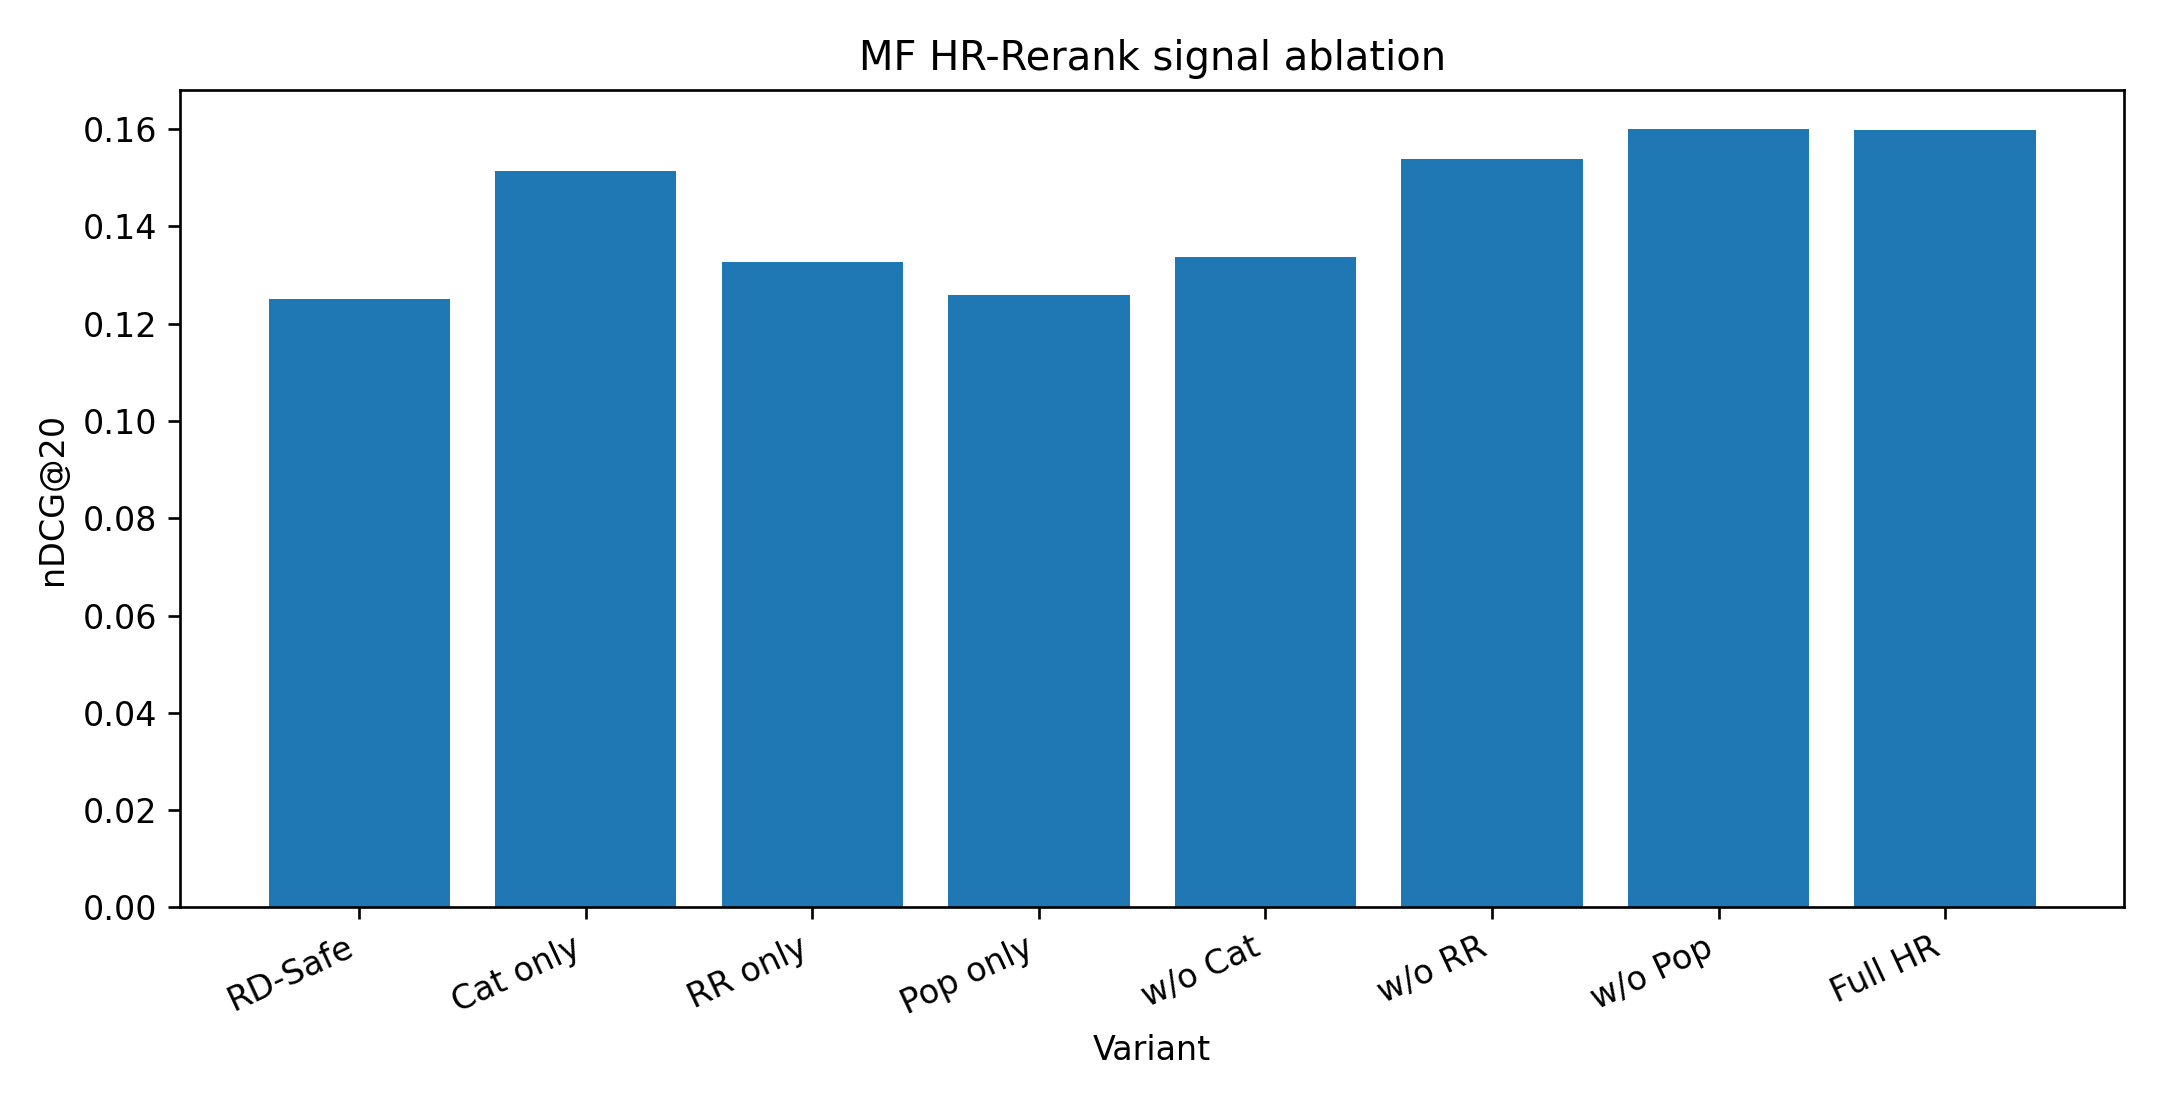
\includegraphics[width=0.92\linewidth]{figures/fig_hr_ablation_mf_ndcg.png}
\caption{MF backbone 上 HR-Rerank 三类信号的消融分析。}
\label{fig:hr_ablation_mf}
\end{figure}


表~\ref{tab:component_ablation} 和表~\ref{tab:hr_ablation} 展示了两层消融结果。主模块消融表明，Original OTC-GW 在 MF 和 LightGCN 上均低于 Target-only，而 RD-Safe 能将性能恢复到安全基线附近，说明可靠性门控能够缓解负迁移。HR 内部消融进一步表明，类别--区域亲和力是最关键的异构关系信号：在 MF 上，仅加入 Cat 就能将 nDCG@20 从 RD-Safe 的 0.1251 提升到 0.1514；去掉 Cat 后，nDCG@20 降至 0.1337。区域共现扩散也能提供一定收益，而区域热度先验更接近弱先验，单独使用时提升有限，且可能引入热门区域偏置。

\subsection{Strict Unseen-pair 鲁棒性分析}

在数据审计过程中，本文发现官方测试集中存在一定比例的 brand-region pair overlap。由于官方划分是按 POI 行切分，同一品牌在同一区域的不同 POI 可能同时出现在训练集和测试集中。为了进一步评估模型对真正未见品牌--区域组合的泛化能力，本文构造 strict unseen-pair 测试集：仅保留训练集中未出现过的测试 brand-region pair，不修改官方训练/测试文件。

\begin{table}[H]
\centering
\caption{官方测试集中 brand-region pair overlap 统计。}
\label{tab:pair_overlap}
\begin{tabular}{lrr}
\toprule
City & Pair overlap & Row overlap \\
\midrule
Chicago & 23.38\% & 25.64\% \\
New York City & 18.39\% & 20.36\% \\
Singapore & 28.91\% & 33.65\% \\
Tokyo & 13.87\% & 14.75\% \\
\bottomrule
\end{tabular}
\end{table}


\begin{table}[H]
\centering
\caption{Strict unseen-pair 鲁棒性分析：四城市平均 nDCG@20。}
\label{tab:strict}
\small
\setlength{\tabcolsep}{3pt}
\resizebox{\linewidth}{!}{%
\begin{tabular}{llcc}
\toprule
Backbone & Method & Official & Strict \\
\midrule
MF & Target-only & 0.1251$\pm$0.0012 & 0.0927$\pm$0.0015 \\
MF & Original OTC-GW & 0.1170$\pm$0.0026 & 0.0876$\pm$0.0025 \\
MF & RD-Safe-OTC & 0.1251$\pm$0.0012 & 0.0929$\pm$0.0016 \\
MF & RD-Safe+HR-OTC & 0.1598$\pm$0.0010 & 0.0943$\pm$0.0010 \\
LightGCN & Target-only & 0.1741$\pm$0.0026 & 0.0964$\pm$0.0020 \\
LightGCN & Original OTC-GW & 0.1291$\pm$0.0029 & 0.0922$\pm$0.0062 \\
LightGCN & RD-Safe-OTC & 0.1719$\pm$0.0016 & 0.0963$\pm$0.0019 \\
LightGCN & RD-Safe+HR-OTC & 0.1738$\pm$0.0047 & 0.0952$\pm$0.0012 \\
\bottomrule
\end{tabular}%
}
\end{table}


表~\ref{tab:strict} 表明，strict unseen-pair 场景下的 nDCG@20 整体低于 official test，说明真正未见品牌--区域组合推荐更困难。尽管如此，RD-Safe 仍能缓解 Original OTC-GW 的负迁移；在 MF 上，RD-Safe+HR 仍略优于 Target-only，而在 LightGCN 上最终方法主要保持接近本地模型的性能。

\subsection{参数与门控分析}

本文进一步统计 RD-Safe 和 HR-Rerank 的门控结果。门控统计结果显示，RD-Safe 在多数情况下选择回退到 Local 或安全候选，说明其核心作用并非强行提高迁移权重，而是阻止不可靠迁移进入最终预测。对于 HR-Rerank，MF 上完整图重排序在 12 个 seed-city 设置中全部通过验证集门控；LightGCN 上则仅有 1 次通过，大多数情况下回退到基础分数。这与主实验结果一致：MF 更依赖外部结构增强，而 LightGCN 已经通过图传播捕获了部分高阶结构。

\begin{table}[H]
\centering
\caption{RD-Safe 与 HR-Rerank 的门控统计。}
\label{tab:gate}
\begin{tabular}{lccc}
\toprule
Module & Backbone & Accept & Fallback/Local \\
\midrule
RD-Safe & MF & 2 & 10 \\
RD-Safe & LightGCN & 1 & 11 \\
HR-Full & MF & 12 & 0 \\
HR-Full & LightGCN & 1 & 11 \\
\bottomrule
\end{tabular}
\end{table}

\subsection{关于 Sparse-OTC 的探索性尝试}

此外，本文曾尝试基于品牌支持度的稀疏性感知迁移策略。该策略的直觉是：低支持品牌更依赖跨城市知识，而高支持品牌更依赖目标城市本地信息。然而实验中发现，仅根据品牌稀疏程度调节迁移强度并不能稳定优于 RD-Safe+HR-OTC。原因可能在于，品牌稀疏性只能描述目标品牌自身样本量不足，却不能判断源城市迁移信号是否可靠；当源城市迁移噪声较大时，提高低支持品牌的迁移权重反而可能放大负迁移。因此，本文最终未将 Sparse 策略纳入最终模型。

\FloatBarrier
\section{相关工作}

\subsection{选址推荐}

选址推荐旨在预测品牌或服务设施适合开设的新位置，在城市计算和商业决策中具有重要价值。早期方法通常依赖地理位置、交通便利性、竞争关系、人口流动等人工设计特征，并多针对少量特定品牌展开。虽然这类方法具有较强可解释性，但依赖高质量细粒度特征，难以扩展到大规模品牌和多城市场景。

近年来，随着推荐系统和图学习方法的发展，研究者开始将协同过滤、学习排序和图神经网络用于选址推荐任务。OpenSiteRec 的提出进一步推动了大规模品牌--区域推荐研究，使模型能够在统一数据集上进行系统比较。

\subsection{跨域与跨城市推荐}

跨域推荐旨在利用源域信息提升目标域推荐效果。跨城市选址推荐可以视为一种特殊的跨域推荐任务，其中不同城市对应不同领域。由于不同城市之间品牌集合、区域集合和商业结构存在差异，直接共享参数或直接迁移交互矩阵通常较困难。因此，如何进行结构对齐和可靠迁移是跨城市推荐中的关键问题。

\subsection{最优传输推荐}

最优传输为跨域分布对齐提供了理论工具。与普通 Wasserstein 距离相比，Gromov-Wasserstein 距离能够在实体空间不同的情况下对齐域内结构，因此适合跨城市品牌和区域表示对齐。OTC 将 GW 最优传输引入选址推荐，通过品牌投影和区域投影将源城市推荐信号迁移到目标城市。本文工作在此基础上进一步关注迁移可靠性和负迁移控制。

\subsection{图结构重排序}

图结构重排序通常在基础推荐分数之上引入额外关系信号，以改善最终排序质量。本文的 HR-Rerank 不是完整异构图神经网络，而是一种轻量级异构关系重排序方法。它利用类别--区域、区域--区域以及区域热度等结构信号，为基础推荐分数提供商业规律补充。

\section{结论与未来工作}

本文围绕跨城市选址推荐中的负迁移问题，对 OTC-GW 框架进行了复现与改进。复现实验表明，无回退 Original OTC-GW 在部分设置下会低于 Target-only，说明跨城市迁移并不总是可靠。为此，本文提出 RD-Safe+HR-OTC：RD-Safe 通过源城市可靠性筛选和安全门控抑制负迁移；HR-Rerank 则进一步利用类别--区域亲和力、区域共现扩散和区域热度先验等商业结构信号增强最终排序。实验结果表明，所提方法在 MF backbone 上显著提升性能，在 LightGCN backbone 上能够有效修复 Original OTC-GW 的负迁移并接近强本地模型。

未来工作可以从以下几个方向展开。第一，可以将源城市可靠性从 city-level 扩展到 brand-level、category-level 或 region-level，以实现更细粒度的安全迁移。第二，若能够获得更丰富的经济和城市特征，例如租金、客流量、消费能力、交通便利性和竞品密度，可以构造更完整的商业异构图。第三，可以进一步改进跨城市对齐机制本身，例如引入 partial OT、unbalanced OT 或置信度感知对齐。第四，可以继续完善 strict unseen-pair 等更严格评价协议，以更准确评估模型在真实新区域推荐场景下的泛化能力。


\begin{thebibliography}{9}

\bibitem{li2024otc}
Xinhang Li, Xiangyu Zhao, Zihao Wang, Yang Duan, Yong Zhang, and Chunxiao Xing.
\newblock Optimal Transport Enhanced Cross-City Site Recommendation.
\newblock In \emph{Proceedings of the 47th International ACM SIGIR Conference on Research and Development in Information Retrieval}, 2024.

\bibitem{li2023opensiterec}
Xinhang Li, Xiangyu Zhao, Yejing Wang, Yu Liu, Yong Li, Cheng Long, Yong Zhang, and Chunxiao Xing.
\newblock OpenSiteRec: An Open Dataset for Site Recommendation.
\newblock \emph{arXiv preprint arXiv:2307.00856}, 2023.

\bibitem{he2020lightgcn}
Xiangnan He, Kuan Deng, Xiang Wang, Yan Li, Yong-Dong Zhang, and Meng Wang.
\newblock LightGCN: Simplifying and Powering Graph Convolution Network for Recommendation.
\newblock In \emph{SIGIR}, 2020.

\bibitem{rendle2009bpr}
Steffen Rendle, Christoph Freudenthaler, Zeno Gantner, and Lars Schmidt-Thieme.
\newblock BPR: Bayesian Personalized Ranking from Implicit Feedback.
\newblock In \emph{UAI}, 2009.

\bibitem{li2022gwcdr}
Xinhang Li, Zhaopeng Qiu, Xiangyu Zhao, Zihao Wang, Yong Zhang, Chunxiao Xing, and Xian Wu.
\newblock Gromov-Wasserstein Guided Representation Learning for Cross-Domain Recommendation.
\newblock In \emph{CIKM}, 2022.

\bibitem{guo2017citytransfer}
Bin Guo, Jing Li, Vincent W. Zheng, Zhu Wang, and Zhiwen Yu.
\newblock CityTransfer: Transferring Inter- and Intra-City Knowledge for Chain Store Site Recommendation based on Multi-Source Urban Data.
\newblock \emph{Proceedings of the ACM on Interactive, Mobile, Wearable and Ubiquitous Technologies}, 2017.

\bibitem{karamshuk2013geospotting}
Dmytro Karamshuk, Anastasios Noulas, Salvatore Scellato, Vincenzo Nicosia, and Cecilia Mascolo.
\newblock Geo-spotting: Mining Online Location-based Services for Optimal Retail Store Placement.
\newblock In \emph{KDD}, 2013.

\end{thebibliography}


\end{document}
